% secciones/02_estado_del_arte.tex
\section{Estado del Arte y Simulación en ROS 2}
La investigación en robótica hospitalaria se apoya fuertemente en entornos de simulación de alta fidelidad. Actualmente, ROS 2 se ha consolidado como el estándar \textit{de facto} debido a su arquitectura distribuida y su soporte para sistemas de tiempo real.

\subsection{Referentes Comerciales: El Robot TUG de Aethon}
\label{sec:tug_aethon}

Uno de los referentes más importantes en la logística interna de centros sanitarios es el sistema \textit{TUG}, desarrollado por \textit{Aethon}. Este robot está diseñado para la automatización del transporte de suministros, medicación y residuos, minimizando la carga física del personal de enfermería.

\begin{itemize}
    \item \textbf{Capacidad de Carga y Tracción:} El TUG destaca por su capacidad de arrastrar carros de hasta $450$ kg, utilizando una base motriz con giro sobre su propio eje (omnidireccionalidad) para maniobrar en espacios críticos.
    \item \textbf{Integración con la Infraestructura:} Se comunica de forma autónoma con el sistema del edificio para gestionar la apertura de puertas y el uso de ascensores mediante protocolos inalámbricos seguros.
    \item \textbf{Seguridad Dinámica:} Emplea una combinación de sensores LiDAR y ultrasonidos para garantizar la detección de obstáculos a diversas alturas, permitiendo una convivencia segura con pacientes y personal médico.
\end{itemize}

\begin{figure}[H]
    \centering
    
    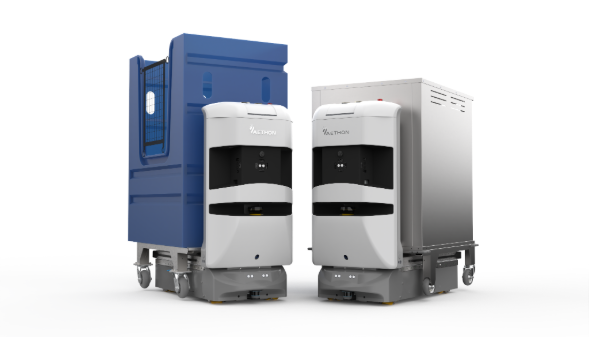
\includegraphics[width=0.7\textwidth]{secciones/images/TUG.png} 
    \caption{Robot TUG de Aethon.}
    \label{fig:robot_tug}
\end{figure}

\subsection{Plataformas de Simulación}
Existen varios repositorios y proyectos destacados que permiten validar algoritmos de navegación y coordinación en hospitales:
\begin{itemize}
    \item \textbf{AWS RoboMaker Hospital World:} Un entorno desarrollado por Amazon que proporciona un hospital completo con habitaciones, quirófanos y pasillos, optimizado para pruebas con Nav2.
    \item \textbf{Open-RMF (Robotics Middleware Framework):} Marco de trabajo para coordinar múltiples robots de diferentes fabricantes en infraestructuras compartidas.
    \item \textbf{Navigation2 (Nav2):} El sistema de navegación de ROS 2 que permite evitar obstáculos dinámicos en tiempo real.

\subsection{Aplicación al Proyecto Actual}
Nuestro diseño de robot mensajero toma la fiabilidad operativa del \textit{TUG} como base, pero evoluciona hacia una solución más ágil. A diferencia de la fuerza bruta del TUG, nuestra propuesta integra una \textbf{suspensión independiente de grado automotriz} y una carga útil optimizada de $25$ kg, facilitando el transporte de muestras biológicas delicadas que requieren una estabilidad superior frente a vibraciones y cambios de dirección bruscos.
\end{itemize}
